\chapter{Conclusão}
\label{cap4}

% \section{Coleta de Dados}

\paragraph{} Foram realizadas diversas simulações para os 71 \textit{Tickers} apresentados na Tabela \ref{tab:5}, durante o período de simulação de 01/01/2019 e 31/12/2021, que inclusive engloba a Crise do Coronavírus ocorrida em março de 2020. O melhor resultado obtido levou em consideração os parâmetros indicados pela Tabela \ref{tab:100}:

\begin{table}[h!]
    \begin{center}
        \begin{tabular}{ c|c }
            Parâmetro & Valor \\
            \hline
            Capital & 100000 \\
            RCC & 0.3\% \\
            \textit{Gain Loss Ratio} & 3 \\
            Menor Risco por Operação & 0.3\% \\
            Maior Risco por Operação & 10\% \\
            Volume Mínimo por Operação & 1 \\
            Venda Parcial & Não \\
            \textit{Stop Loss} & Normal \\
            Descanso após Operação de Sucesso & Não \\
            Descanso após Operação de Falha & Não \\
            Normalização por Frequência de Operações & Sim \\
            Compensação por Lucratividade & Sim \\
            Descanso por Identificação de Crises & Sim \\
            Descanso por Tendência de Baixa & Sim \\
            RCC Dinâmico & Sim \\
            RCC Dinâmico (Referência) & 100\% \\
            RCC Dinâmico (K) & 5 \\
        \end{tabular}
        \caption{Configurações de Simulação}
        \label{tab:100}
    \end{center}
\end{table}

\paragraph{} As Figuras \ref{fig:300} e \ref{fig:301} mostram a performance da carteira em comparação ao Baseline, iBovespa e CDI acumulado no período, assim como os valores métricas resultantes dessa performance.

\begin{figure}[h]
    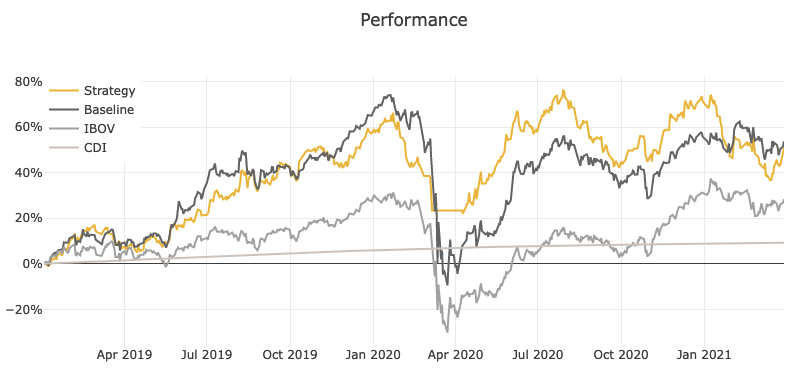
\includegraphics[scale=0.52]{resultado_final.png}
    \centering
    \caption{Performance da Carteira}
    \label{fig:300}
\end{figure}

\begin{figure}[h]
    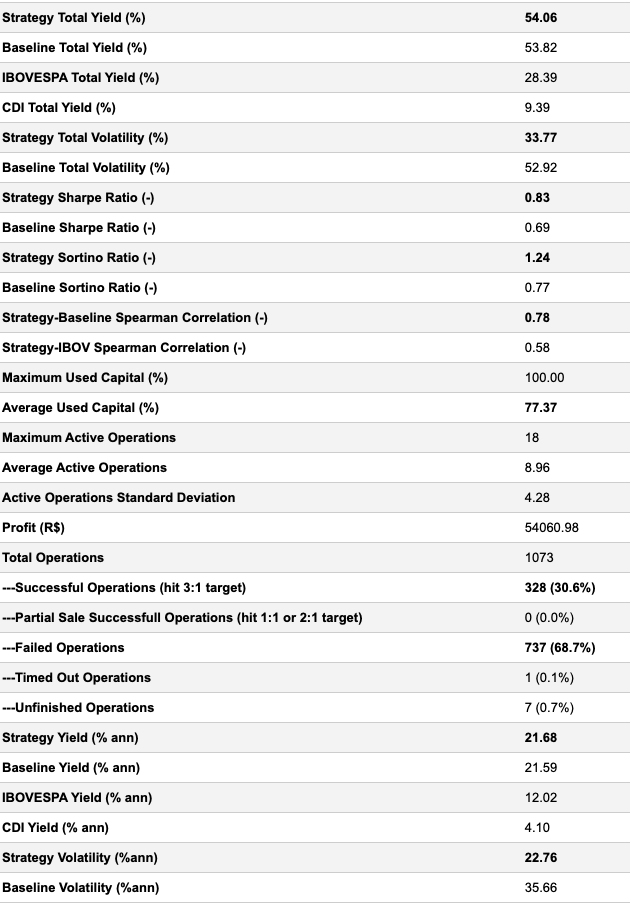
\includegraphics[scale=0.60]{resultado_valores.png}
    \centering
    \caption{Resultados}
    \label{fig:301}
\end{figure}

\paragraph{} Analisando a Figura \ref{fig:300}, pode-se perceber que (FAZER COMENTÁRIOS). Quanto aos resultados mostrados na Figura \ref{fig:301}, (FAZER COMENTÁRIOS).

\paragraph{} (Mostrar gráficos de operações por ticker).